%! Author = topihdez
%! Date = 02/03/22

% Preamble
\documentclass[11pt]{article}
\usepackage{graphicx}
\graphicspath{ {./} }

% Packages
\usepackage{amsmath}

\title{Linear Regression models comparison}
\author{Topiltzin Hernández Mares}

% Document
\begin{document}
\maketitle

\begin{abstract}
    Linear regression models can be easily implemented given its simplicity to program and test.
    But if an improvement in the performance and predictions is required, then a number of enhancements are needed in
    the model, such as hyperparameter optimization and data normalization.
\end{abstract}

\section{Model Description}\label{sec:model_description}
    In the last year, the \textbf{LinearRegressionGD} model was implemented as a class project.
    In this model, the cost function optimization was done with \textbf{Gradient Descent (GD)}, and it remains the same.
    The \textbf{GD} was implemented with help of matrix multiplications using the library \textbf{numpy} in order to
    improve the performance of the model.
    Other than small optimizations on the multiplication of some numbers, the model stays the same as the original
    implementation.

\section{Data Processing}\label{sec:data_processing}
In this section of the model is were most of the improvements are located. In the following subsections the changes are
going to be described in detail, with a reason of why were needed.

\subsection{Original Model}
    In the original model, the data processing process was really simple, this were the steps:
    \begin{enumerate}
        \item The data is extracted from the insurance.csv file.
        \item All the non-smoker registers are removed from the dataframe.
        \item The dataframe is divided into train and test data.
        \item Both dataframes (train and test) are "normalized" with a simple multiplication to escalate the values.
        \item Finally, when a prediction is needed, the scaling process is reverted with the predicted values.
    \end{enumerate}

    With the raw data (unscaled), the model, even with a small learning rate, diverged easily with a few hundred
    iterations. This is why the scaling was needed. In the original implementation, the scaling is simple because of
    lack of time in the development of the model. In this second iterations, the main objective was to improve the
    scaling of the data to improve the training process.

\subsection{New Model}
    After learning more about data scaling and normalization, the new data processing steps are the following:
    \begin{enumerate}
        \item The data is extracted from the insurance.csv file.
        \item All the non-smoker registers are removed from the dataframe.
        \item The \textit{min-max} normalization method is applied to the cleaned dataframe.
        \item The dataframe is divided into train and test data.
        \item Finally, when a prediction is needed, the normalization process is reverted with the predicted values.
    \end{enumerate}

    In the following sections, the improvements on the model is going to be explained in detail, but it can be said that
    the normalization method implemented in this new iteration improved the quality of the predictions.

\section{Evaluation}
    Since this is a linear regression model, there are two main metrics that are easily comparable:
    \textit{Mean Squared Error (MSE)} and \textit{Coefficient of Determination (R2)}. These two metrics will be measured
    from the train and test processes from both models.

\subsection{Method}
    For measuring both metrics for both models, it was decided to implement a script in order to simplify the process.
    The script \textit{measure.py} was written, along with helper functions to reduce code duplication in the different
    training scripts for each model.

    In this script, each model is trained 100 times, measuring each \textit{MSE} and \textit{R2} in each iteration. In
    every training, the number of learning iterations for the model was increased by 200. This was done in order to
    know the learning behavior of both models.

\section{Results}\label{sec:results}
    After executing the experiment, the metrics were obtained correctly and the comparison between the two models was
    possible.
    \begin{figure}[h]
        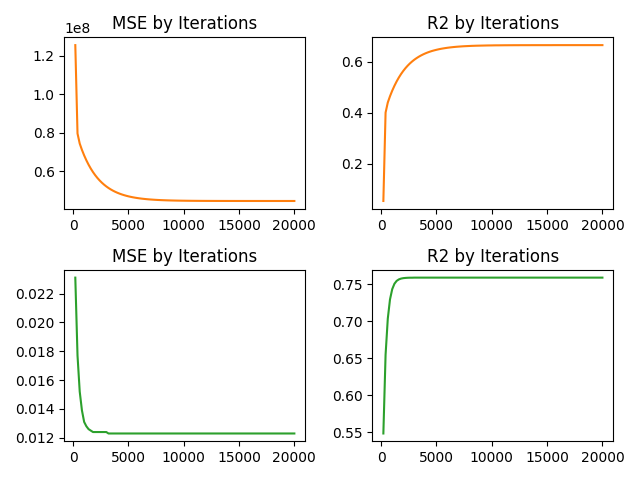
\includegraphics{figures}
        \caption{
            \textit{MSE} and \textit{R2} from both models in training process. Old model (orange) and new model (green).
        }
        \label{fig:results}
    \end{figure}

    As can be seen in Figure \ref{fig:results}, the new model has a faster learning behavior, since the \textit{MSE} and
    \textit{R2} reach their minimum much faster than the old model. It is also important noting that new the \textit{R2}
    is much better than the one from the old model, this means the predictions are more accurate in the new model.

\section{Conclusions}
    As can be seen in the Results section, the new model makes better predictions, this is because the data processing
    in this model is better than a simple scaling. When using data normalization, we allow our model to fit better to
    the training data and make more accurate predictions.
\end{document}